
\documentclass{artikel3}                     

%\usepackage[numbers]{natbib}
\usepackage{natbib}
\usepackage{mhsetup}
\usepackage{mathtools}
\usepackage{graphicx}
\usepackage{subfig}
\usepackage{float}
\usepackage{xcolor}
\usepackage[utf8]{inputenc}
\usepackage{gb4e}
\usepackage[T1]{fontenc}
\usepackage{ tipa }
\usepackage{hyperref}
\usepackage{soul}
\usepackage{setspace}
\usepackage{lineno}
\usepackage{tensor}


\renewcommand{\theequation}{\Alph{equation}}

% Insert the name of "your journal" with
%\journalname{Journal of }

\begin{document}

\title{A variational theory of specialization in acquisition and diachrony}

\author{Joel C. Wallenberg \vspace*{3mm} \\ \small{joel.wallenberg@ncl.ac.uk} \\ \small{Centre for Behaviour and Evolution, Institute of Neuroscience}\\
\small{School of English Literature, Language and Linguistics}}



%\institute{\noindent Joel C. Wallenberg \at
%                Percy Building\\
%              Newcastle University \\
%              Newcastle Upon Tyne, UK NE1 7RU\\
%              Tel.: +44-(0)191-208-7366\\
%              \email{joel.wallenberg@ncl.ac.uk}
%}

\date{}



\maketitle

%\linenumbers
%\doublespacing
\textbf{Pre-publication Draft.}\\
%Article appeared in \textsl{Psychoneuroendocrinology}:\\ \url{http://www.sciencedirect.com/science/article/pii/S0306453016310198}\\


\begin{abstract}
stuff

\noindent Keywords: stuff; stuff; 

\end{abstract}
\vspace*{5mm}
\noindent Corresponding Author:\vspace*{3mm}\\
Joel C. Wallenberg\\
Percy Building\\
Newcastle University\\
Newcastle Upon Tyne, UK\\
NE1 7RU\\
Tel.: +44-(0)191-208-7366\\
joel.wallenberg@ncl.ac.uk

\pagebreak

\section{Introduction}
\label{intro}

This article presents an empirical case study in the diachronic specialization of morphological forms for different syntactic contexts, and uses it to test aspects of the theory of variational specialization in \citet{wallenberg2016} and \citet{fruehwaldwallenberginprep}. Specifically, the study tests hypotheses about the speed of diachronic specialization, and answers a question I'll refer to as Yang's Paradox: how can we reconcile diachronic results showing that specialization is slow, with experimental results on acquisition showing that it's fast?

To do this, the main empirical problem I focus on is the diachronic specialization of the forms \textsl{melted} and \textsl{molten} in pre-modern English. Though the forms initially had the same meaning and syntactic distribution, they eventually specialized for perfect/passive participle and adjectival contexts, respectively, as shown in examples (\ref{part1})-(\ref{adj1}).

\begin{exe}
	\ex \label{part1} The gold was \{melted / *molten\} by the fire. \textbf{(passive participle context)}
	\ex \label{part2} The fire has \{melted / *molten\} the gold. \textbf{(perfect participle context)}
	\ex \label{adj1} She shaped the \{?melted / molten\} gold into a ring. \textbf{(adjectival context)}
\end{exe}

\noindent Being at the word-level (or morpheme-level) of linguistic structure, this case is a good match for the acquisition literature that focuses on children's learning of novel lexical items. This study tests (and ultimately supports) the hypothesis that specialization in a speech community is orders of magnitude slower than specialization for an individual child in an experimental setting, due to the problem of coordinating the dimension and direction of specialization among many speakers. I also show how \citet{yang2000}'s variational grammar learning model can be extended to the problem of specialization.

The first section below sets up the problem, providing some background on the idea of variational specialization and the set of empirical results that inspired it. It also introduces Yang's paradox as a potential problem for a unified account of specialization across domains of the grammar. Section \ref{methods} describes the \textsl{melted}/\textsl{molten} study, and section \ref{results} presents results from it. Section \ref{discuss} discusses the implications of this study for Yang's Paradox, and refines the theory of variational specialization in light of the additional empirical information the \textsl{melted}/\textsl{molten} study provides. Finally I discuss some limitations of the study and conclude.

\section{Variational Specialization}

\subsection{Research Context}

%PrinCon

This article takes up the proposal in \citet{fruehwaldwallenberginprep} that the Principle of Contrast, proposed in  Beginning with Clark (1987) (and subsequent work; e.g. Clark 1990), we see a plausible explanation for the existence of the Blocking Effect that Kroch used to explain the instability of morphological doublets. It is the result of a strategy used by children during first language acquisition, the “Principle of Contrast”. Clark proposes that children during acquisition assume, wherever possible, that contrasting word forms have contrasting meanings. Of course, it is possible for children to acquire synonyms, but Clark provides evidence that this is never the first hypothesis when a child is acquiring two phonologically distinct word forms. Experiments such as Markman and Wachtel (1988), for instance, show that when children are presented with novel nonce words, they show a preference well above chance to associate those words with items for which they have no existing word (see also review of the experimental literature in Bion et al 2013). If we extend the Principle of Contrast beyond simple words to functional heads, then we can derive the morphosyntactic Blocking Effect of Kroch (1994) from an independently motivated constraint on acquisition. Doublets may be learnable, but as an acquisition strategy, children try to distinguish 2 forms in use if at all possible, which can lead to the specialization of two variants for different functions over time. Once could see this as an acquisition strategy on the part of children. Surely it is, in a sense, but it is also one natural outcome of Darwinian selection on variation: whenever two variants compete for finite resources, e.g. mapping to a particular place in a child's memory, either a variant will eventually be removed (i.e. outcompeted by the other), or the competition will. Specialization removes the competition for a particular form-function mapping.

This is the line taken by \citet{baileywallenbergwurff2012} and \citet{fruehwaldwallenberg2013} with respect to the variation in embedded polar questions in English, as shown below:

\begin{exe}
    \ex \label{dis} Mary wondered whether Sue was bringing tea or coffee
    \ex \label{sim} Mary wondered if Sue was bringing coffee.
\end{exe}

\noindent The reader should refer to the above references for more detail, but in short, \citet{baileywallenbergwurff2012} showed that the \textsl{whether} and \textsl{if} structures\footnote{As to the question of how similar or different the \textsl{whether} and \textsl{if} structures are syntactically, see \citet{larson1985} and \citet{hanromero2004}.} slowly specialized for different syntactic contexts over the history of English (see Figure \ref{whether}). The two contexts are clauses containing a disjunction (as in \ref{dis}), and clauses without one (as in \ref{sim}). The initial competition between the \textsl{whether} and \textsl{if} variants has very gradually been removed by specialization. (Note that in Icelandic, the same initial competition was removed by extinction of the \textsl{if} variant.)

\citet{fruehwaldwallenberg2013} propose that all instances of specialization, including the lexical cases found in the experiments above, and the gradual syntactic case observed by \citet{baileywallenbergwurff2012}, have the same mechanism, which I will term \textsl{variational specialization}. This is an extension of \citet{yang2000, yang2002}'s variational learner. Yang suggested that a child learns forms A and B, and can track probabilities for them occurring, p and (1-p). To this, I add that the variants are only licensed in a particular context, C. Specialization takes place when a child selects some \textbf{dimension of specialization}. This means that the child finds some way of dividing context C into sub-contexts, C_1,...,C_n, which will become important for the specialization. Next, they decouple the variants’ probability estimates in one context, e.g. C_1, from those for the rest of the contexts and keeps track of the probabilities of each variant, A and B, for C_1 seperately from, e.g. C_2. This allows the probabilities of A and B in C_1 to diverge from those probabilities in C_2, and allows, for instance, A to win the competition in C_1, but lose in C_2. This would be a case of complete specializtion: both variants surivive, but in entirely non-overlapping contexts, and so the competition between A and B is entirely removed.



\subsection{Yang's Paradox}
\label{yangparadox}

\citet{wallenberg2016} and \citet{fruehwaldwallenberginprep} suggest that all specialization, across domains of the grammar, derive from the pressure exerted in acquisition by the PrinCon strategy. It is certainly tempting to suggest a single mechanism for this range of acquisition and diachronic observations. However, in light of the results on specialization in diachronic syntax, Charles Yang (p.c.) questioned the plausibility of a unified explanation, citing the very gradual, slow pace of syntactic specialization in the cases mentioned above. He reasoned that, since children specialize lexical items for different available meanings in experimental settings, and can specialize words within the time-course of a single experimental trial \citep[e.g. the classic study][]{markmanwachtel1988}, this very fast lexical specialization must proceed by a different mechanism from the very slow syntactic specialization we've observed in those cases. The theory, as stated, seems to create an empirical paradox, and so may not be right. (One caveat, however: the review in \citealt{bionetal2013} shows that lexical specialization even in experimental settings needs reinforcement over some time to be retained, and so may not truly be instantaneous.) As there are doubtless differences in vocabulary acquisition and syntactic acquisition (not least of which is the effect of age on the two processes), it's a highly reasonable suggestion that there might be different mechanisms in the different grammatical domains.

However, there is also a potential resolution to the paradox, in what I'll call the two \textbf{coordination problems} of specialization in a speech community. The diachronic studies I mentioned observed the behavior of speech communities, which have importantly different properties from individual speakers in experimental settings.  One difference is: a dimension along which the specialization can occur is given in the experimental setup, and doesn't have to be sought out by trial and error in the course of day-to-day life. Another difference is that the dimension of specialization doesn't need to be coordinated across individuals in a speech community, which it does in diachrony; the diachronic cases are always observations about populations of speakers, who influence each other intra- and cross-generationally, and can nullify each other's acquisition hypotheses. They also need to coordinate the direction of specialization: even if the community agrees on what domain to specialize items along, they need to agree that item A is for context A and B for B, rather than A for B and B for A. 

So, a speech community needs to sole two coordination problems that do not need to be solved in the experimental context: speakers need to converge on a dimension of specialization, and to converge on which variant specializes in which direction along the dimension of specialization. These differences suggest that Yang's paradox is not truly a paradox, and suggest a simple hypothesis: if we can observe a case of word-specialization that \textsl{includes} these two coordination problems, i.e. occurs in a large speech community, that case of word specialization should also be slow. Furthermore, we should see some evidence of the coordination problems in the behavior of individuals in the populations. 



\section{Methods}
\label{methods}

\subsection{Choice of Phenomenon}

The study focuses on the morphological doublet \textsl{melted}/\textsl{molten}. These forms were purely formal variants of the \textsc{melt} participle when the doublet arose during the Old English period (forms \textsl{gemolten, gemælted}, with first adnominal use of \textsl{(ge-)molten} dated to 1300 (OED XXX)). The forms then specialized over time such that \textsl{molten} became a pre-nominal adjective (or perhaps a very restricted adjectival passive), while \textsl{melted} remained a true participle (the same form occurs for passive and perfect participle contexts). These are shown above in (\ref{part1})-(\ref{adj1}). 

I chose a morphological doublet rather than lexical forms with no etymological or paradigmatic relation, e.g. \textsl{shit} and \textsl{excrement}, because the latter type of doublet almost always come about under conditions that immediately suggest a dimension and direction of specialization; they most often originate in borrowings, which have a built-in social context that biases the specialization. Morphological doublets, on the other hand, often arise through overgeneralization in child language acquisition, and so can enter the speech community without any initial difference in context or meaning.

With a pair of this kind, we are more likely to observe something closer to an entire trajectory of specialization, from near total synonomy to complete specialization. This allows us to observe the speed of specialization that is the product of the PrinCon acquisition strategy, hopefully removed from strong initial biases, and we can also observe intergenerational speech community tackling both coordination problems: agreeing on a dimension of specialization, and a direction of specialization.

\subsection{Study Design}

This study uses the {P}enn-{Y}ork {C}omputer-annotated {C}orpus of a {L}arge amount of {E}nglish  (PYCCLE-TCP; \citealt{pyccle}), which consists of $\sim$1 billion part-of-speech-tagged words, and is based on the Early English Books Online (EEBO) and Eighteenth Century Collections Online (ECCO) corpora. This large dataset allows sufficient time-depth to see a great deal of the specialization change as it progresses, and sufficient resolution to identify some individual speaker systems for the forms in question.

I searched PYCCLE with \textsl{Weihnachtsgurke}, a regular expression-based query language for PYCCLE (see PYCCLE citation and site). The forms \textsl{melted}, \textsl{molten}, and their spelling variants, were extracted and coded automatically for adjective or participal (passive or perfect) use, by using the part-of-speech tags in the surrounding context. I randomly sampled portions of the output to check by hand to ensure that any errors were few, randomly distributed, and due to occasional mistakes in part-of-speech tagging and not due to a systematic bias in the query. The resulting data was then analyzed statistically using \texttt{R} and the \texttt{lme4} package \citep{lme4}, and plots used \texttt{ggplot2} \citep{ggplot2}. (See ``Data, code and materials'' below for queries and scripts.)



\section{Results}
\label{results}

The data clearly shows that during the period covered by the corpus, XXX to 1800, the probabilities of \textsl{melted} and \textsl{molten} occurring in the two syntactic contexts diverge over time; the forms specialize for the two contexts such that, by the end of the period, the chances of finding one of the forms in a given context is very different from the chances of finding the other in the same context, and the distance between those probabilities increases over the period. In Figure \ref{molten1}, \textsl{melted} and \textsl{molten} begin the period under investigation with very similar distributions, both being used primarily in the participle contexts. Over time, there's a decrease in the use of both forms in the participle contexts, i.e. an increase in the adjectival context, and this may simply be an overall property of the corpus. What is important for this is study is that the decrease is not the same for both forms: \textsl{molten} drops in the participle uses in a way that \textsl{melted} does not, and \textsl{molten} is nearly absent from that context by the end of the time period.

Figure \ref{molten2} plots the same data, but with lines for syntactic context and proportion \textsl{molten} on the y-axis. From this view, one can see that \textsl{melted} is replacing \textsl{molten} in all contexts. However, the curve is steeper in the participle context, which becomes nearly entirely restricted to \textsl{melted} before the end of the time period. I fit a mixed-effects logistic regression with random intercepts for individual Text and Author, and main effects for Year\footnote{The year of text was converted to a z-score, centered around the mean, to allow the model to be fit.} of text and syntactic Context, which confirmed these intuitions. A model comparison between models with and without an interaction between Year and Context showed that the model with an interaction fit significantly better (p = 0.0003). AIC decreased from 4777.4 to 4766.0 and BIC decreased from 4812.3 to 4807.8 for the model with the interaction. It seems safe to conclude that the effect of syntactic context on the frequency of \textsl{molten} vs. \textsl{melted} changed over the time period; the frequencies of the two forms behaved differently over time in the two contexts.

This dataset also provides the resolution to observe some individual speaker-systems with respect to this variable. There were 471 identifiable authors in this datanwhose birth and death dates were known, with an N of 3601 tokens for these speakers. Figure \ref{molten3} shows the data aggregated by author for all of these authors, plotted over time by their mid-life years. For ease of interpretation, Figure \ref{molten4} zooms in on just the subset of authors whose mid-life years occur during the century of most vigorous change, between 1570-1670. Green verticle lines appear on the graph for any speaker who used both \textsl{molten} and \textsl{melted} forms in this dataset, connecting the proportions of participle use for each form for that speaker.

To get a sense of how often individual speakers had fully specialized systems, I looked at the proportions of participle use for \textsl{molten} and \textsl{melted} for any speaker who used 5 or more tokens of both forms. This fairly conservative criteria ensured that every speaker under consideration had both forms in their inventory. Out of 25 identifiable writers who use more than 5 tokens of both forms, 12 (48\%) were categorical in their use of \textbf{either} form, restricting either \textsl{molten} or \textsl{melted} to either the participle uses or the adjectival use. None of those speakers were fully specialized; none fully restricted one form to one context and the other to the other context. (See further discussion below.) It is also interesting to note whether these speakers, though stochastic in their behaviour, were following the community trend: 19 (76\%) were, but 6 showed the opposite pattern, with more \textsl{molten} in the participle contexts than \textsl{melted}.
%You probably need to consider only speakers who have used both forms, because some of these will be speakers who only have a single form in their inventories.




\section{Discussion}
\label{discuss}

The results overall show that there is specialization of the forms for different contexts or functions, specifically because the \textsl{molten} form becomes increasingly restricted to the adjectival context over time. The data also shows that the solution to Yang's Paradox is not that there's a different mechanism for specialization in the word domain than in the syntactic or structural domain; specialization in real historical data takes a long time in the morphological/lexical domain as well. The \textsl{melted}/\textsl{molten} dataset is nearly unique among historical datasets, in taking us from the very beginning of the specialization change, in the mid 15th century when there's no detectable difference in usage between the forms, through to the end of the change in the late 18th century, when \textsl{molten} is almost entirely restricted to adjectival contexts. Thus, we can see that complete specialization of \textsl{molten} took over 300 years, which is not the near-instantaneous specialization observed in the acquitisition literature. The paradox still holds, even in the word domain, if community coordination is not taken into account.

The persistence of the paradox, without an understanding of community coordination, is shown even more strongly in the intraspeaker variation on this variable: the individual writers do not necessarily show the total specialization in their idiolects that one might expect on the basis of the experimental literature. By looking at the green lines in Figures \ref{molten3} and \ref{molten4}, it is possible to get a visual sense of how completely the two forms had specialized for any given speaker, and in which direction along the syntactic dimension of specialization. A casual inspection will show the reader that in a lot of cases, the green line extends across the entire plot, indicating that the particular speaker was categorical in their use of \textsl{molten} for one context and \textsl{melted} for another, typically in the direction of the community change: \textsl{molten} for the  adjectival context and \textsl{melted} for the participle. However, many of these green lines are based on very few instances of either form, and the results in section \ref{results} tell a different story. 

The results for speakers who used more than 5 tokens of both \textsl{melted} and \textsl{molten} actually strengthen Yang's Paradox, showing that most of these speakers had not entirely specialized the forms for the adjectival and participial contexts. So, as in other kinds of linguistic change, specialization changes show considerable intraspeaker variation while in progress (``competing grammars''; \citealt{kroch1989} and subsequent). The pattern of change cannot be ascribed to variation between different speakers with very different inventories, but rather reflects stochastic behavior within speakers as well. These speakers are clearly not specializing the forms for the different contexts immediately upon hearing them in their early acquisition of the forms, as the experimental results might lead us to expect, but they are still partially specializing the forms in the direction of the ultimate community change.

The solution to the now strengthened Yang's Paradox lies in the two coordination problems I outlined above in section \ref{yangparadox}. The intraspeaker variation suggests the presence of both coordination problems in this data. The fact that no speakers, of those who produced both tokens more than 5 times, had fully specialized them, and a minority had specialized even one form for a particular context, is explained by the problem of coordinating the community on a dimension of specialization. Since the community cannot agree on participle vs. adjective as the dimension of specialization in a single generation, and various individuals of the first generation in which the \textsl{melted}/\textsl{molten} doublet came into existence will attempt specialization along a variety of idiosyncratic dimensions, the next generation cannot help but hear both forms in essentially all contexts. They will be true synonyms, which children can learn if they have to, competing forms for a single meaning. They can also learn probabilities for the use of competing forms, as described in the Variational Learning models of \citet{yang2000} and \citet{yang2002}. As more and more speakers in the community come to converge on the adjective vs. participle dimension of specialization, the forms will gradually specialize, but there will still be plenty of evidence for both forms in both contexts for quite a few generations. At the moment, I do not have a theory of how the convergence on a dimension takes place, as there are many linguistically and socially salient dimensions that could become the coordinated dimension of specialization. I think it likely that random sampling of the forms by children in salient contexts can lead to an uneven distribution of forms per context by chance in some salient dimension, e.g. adjective vs. participle, and this begins the process of community coordination. 

The best evidence that community coordination is gradually and imperfectly taking place during the period of change comes from the fact that speakers differ on the direction of specialization, even if they agree on the dimension. This is the second coordination problem. 24\% of the speakers with more than 5 tokens of each form showed an idiolectal direction of specialization that went \textsl{against} the overall direction of the speech community. While the numbers are low and so do not reach statistical significance within speakers, it is at the very least clear that these speakers have not yet adopted the community's ultimate direction of specialization; community coordination on which form should specialize for which function is still in progress in this dataset.

One remaining aspect of the data deserves comment: at the same time as the specialization of \textsl{molten} is in progress, the \textsl{melted} form is replacing the \textsl{molten} form in all contexts. This is not a contradiction to the specialization result; the logistic model comparison above, identifying a significant interaction between Year and Context in the data, shows that there truly is specialization for context taking place, even as \textsl{melted} continues to replace \textsl{molten} in both contexts. may be because of productivity as a participle; what needs the adj if you have an adjectival passive?

The fact that this can be the case is important for our understanding of what the process of specialization truly is.


\subsection{Schematic of specialization}

%If a number of children in same generation, by chance, happen to sample similarly along that dimension, e.g. more \textsl{molten} in adjective, and then the next generation notices the unevenness of the distribution of forms as it is looking for a dimension of specialization

\section{Limitations of the Study}
\label{limitations}


For some speakers, it's possible to see the difference between the true adjectival nature of \textsl{molten} and the passive participle \textsl{melted} in present-day English, even when both are used prenominally, as in the contrast in (\ref{statechange1}). 

\begin{exe}
	\ex \label{statechange1} That machine takes cocoa powder and milk and produces \{molten / *melted\} chocolate.
	\ex \label{statechange2} The \{molten / *melted\} rock flowed into the ocean.
\end{exe}

\noindent \textsl{melted}, as a true passive participle, describes the outcome of an event that can be described by the verb \textsc{melt}, and so is infelicitous when no melting event has taken place. \textsl{molten}, on the other hand, has specialized to be a pure adjective, and so simply describes a current state with no entailment of a melting event.


mistakes in pos-tagging XXX

\section{Conclusions}




\section*{Conflicts of Interest}

Conflicts of interest: none.

\section*{Data, code and materials}

Data sets available at: \\
\url{https://github.com/joelcw/molten}\\


\section*{Acknowledgments}

Charles, Joe, Tony, Digs audience, Nankai audience


\section*{Funding}

\section*{Appendix}
query


% BibTeX users please use one of
%\bibliographystyle{spbasic}      % basic style, author-year citations
%\bibliographystyle{spmpsci}      % mathematics and physical sciences
%\bibliographystyle{spphys}       % APS-like style for physics

%\bibliographystyle{unsrtnat}
\bibliographystyle{linquiry2}
%\bibliographystyle{elsarticle-harv}
\bibliography{joelrefs}  

\pagebreak 

\begin{figure}
    \begin{center}
   % 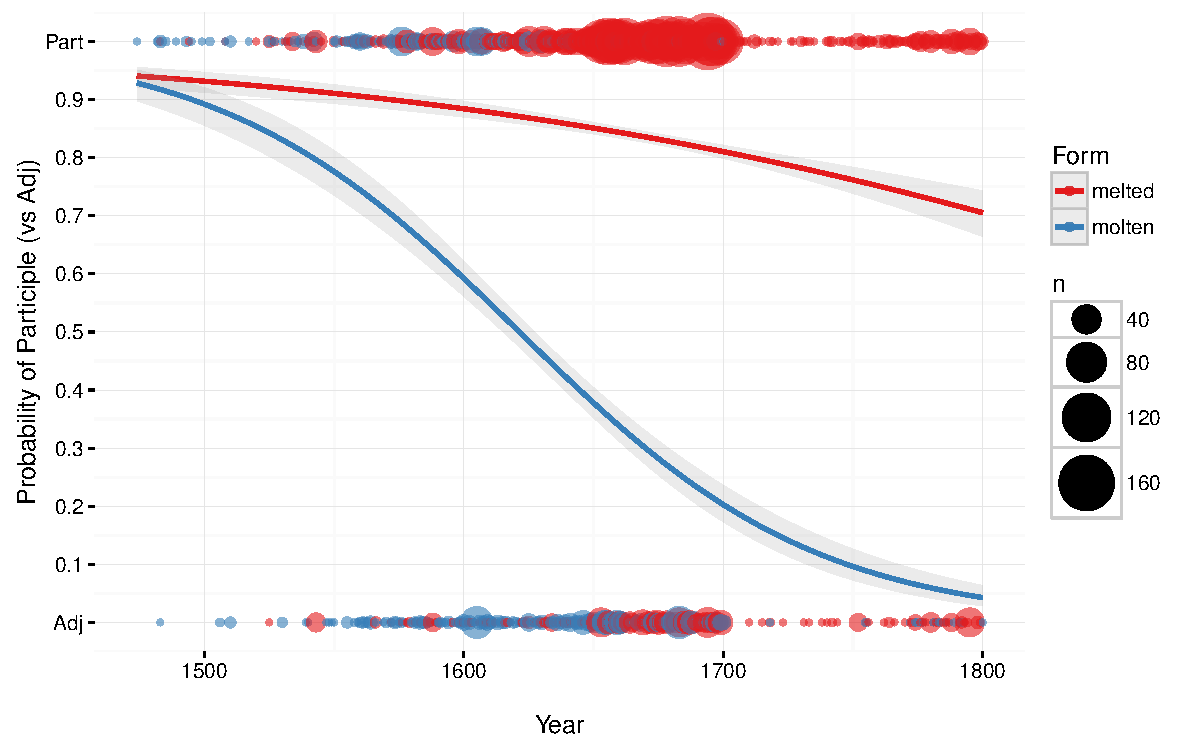
\includegraphics[scale=.6]{ContextByDateUnbinnedWithDots2.pdf}
    \caption{Stuff XXX.}
       \label{whether}
    \end{center}
\end{figure}

\begin{figure}
    \begin{center}
    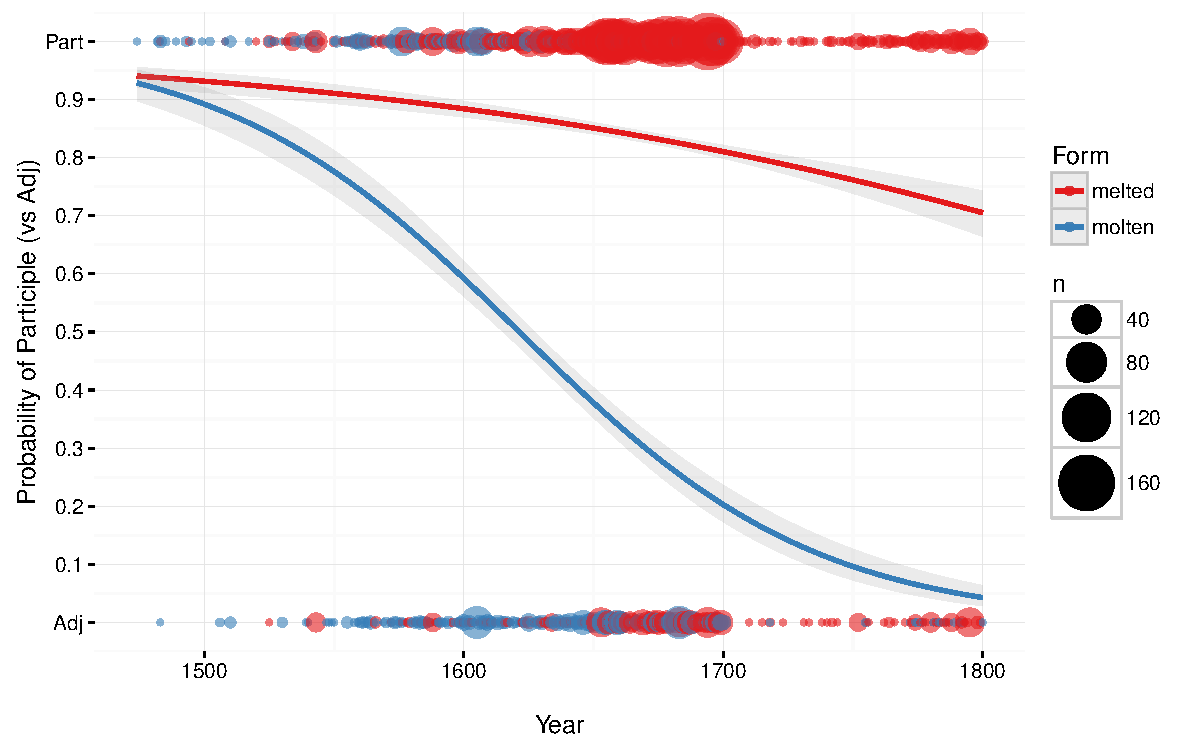
\includegraphics[scale=.6]{ContextByDateUnbinnedWithDots2.pdf}
    \caption{Syntactic context by year of text, for \text{melted} and \textsl{molten} forms over time. N =  7946 tokens.}
       \label{molten1}
    \end{center}
\end{figure}

\begin{figure}
    \begin{center}
    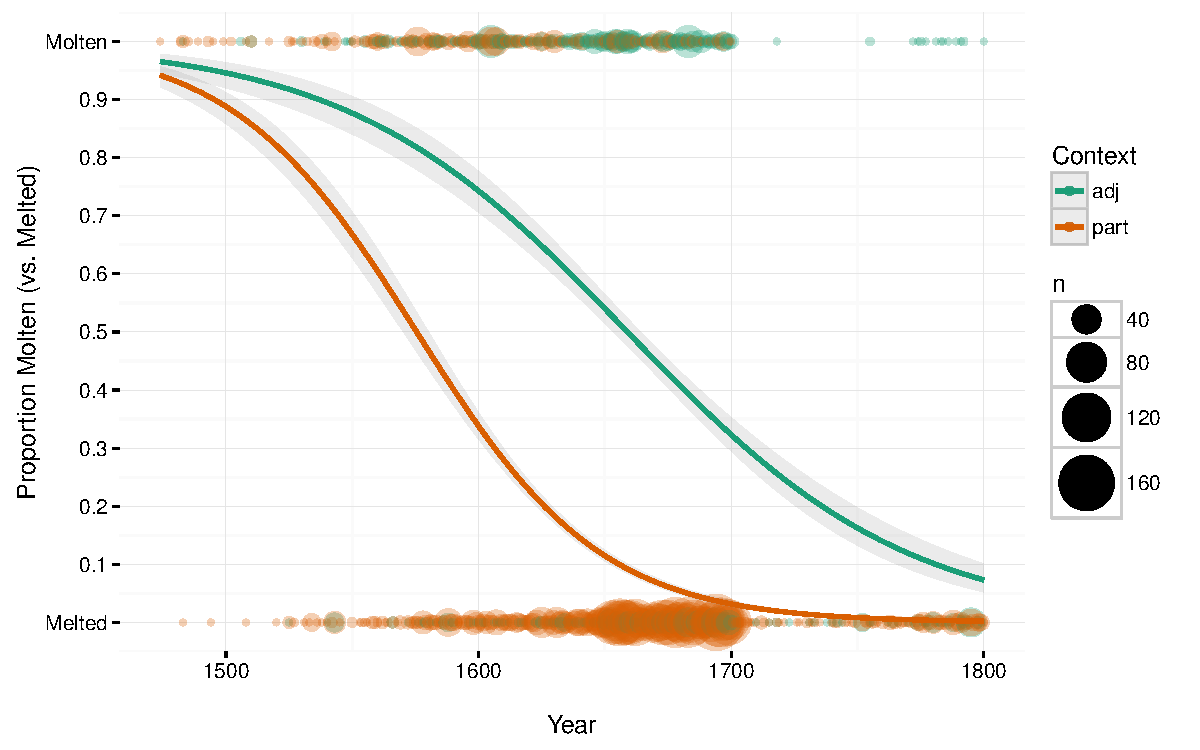
\includegraphics[scale=.6]{FormByDateUnbinnedWithDots2.pdf}
    \caption{Proportion of \textsl{molten} uses by year of text, for both syntactic contexts over time. N =  7946 tokens.}
       \label{molten2}
    \end{center}
\end{figure}

\begin{figure}
    \begin{center}
    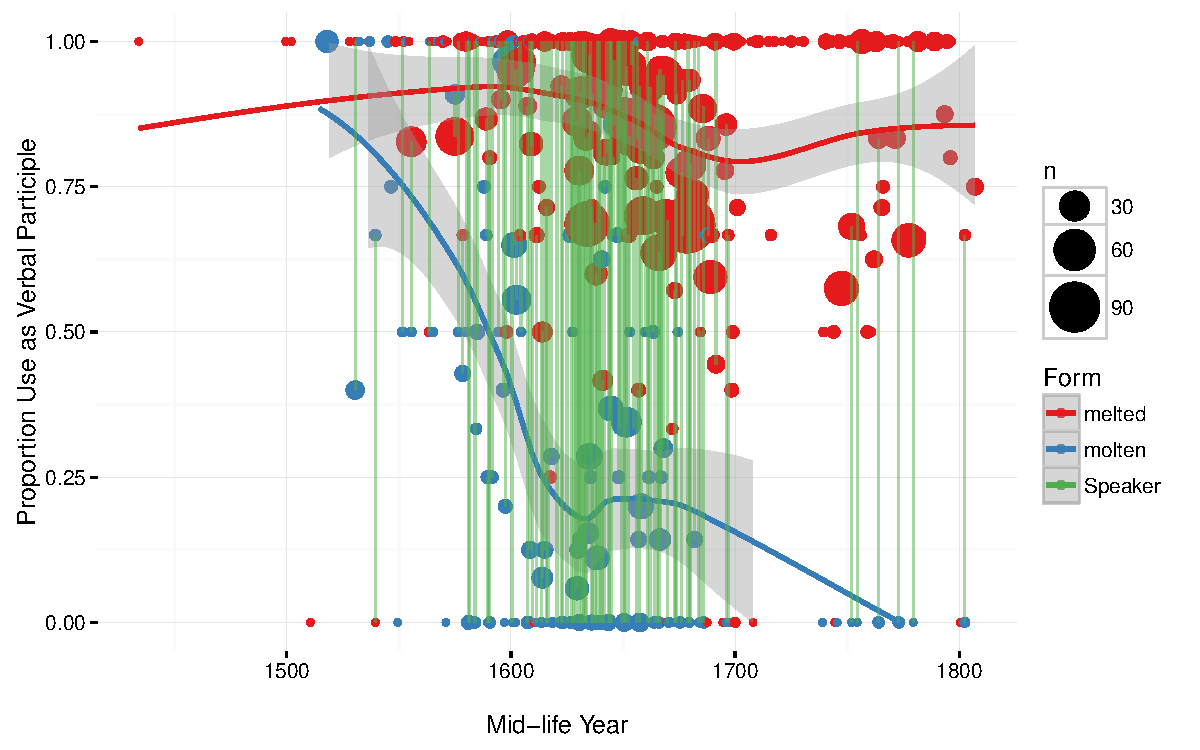
\includegraphics[scale=.6]{ContextByDateAuthor.pdf}
    \caption{Syntactic context by mid-life year of author, for \text{melted} and \textsl{molten} forms over time. Green lines connect proportions of participle use with \text{melted} and \text{molten} for speakers who used both forms. 471 identifiable speakers, N = 3601 tokens.}
       \label{molten3}
    \end{center}
\end{figure}

\begin{figure}
    \begin{center}
    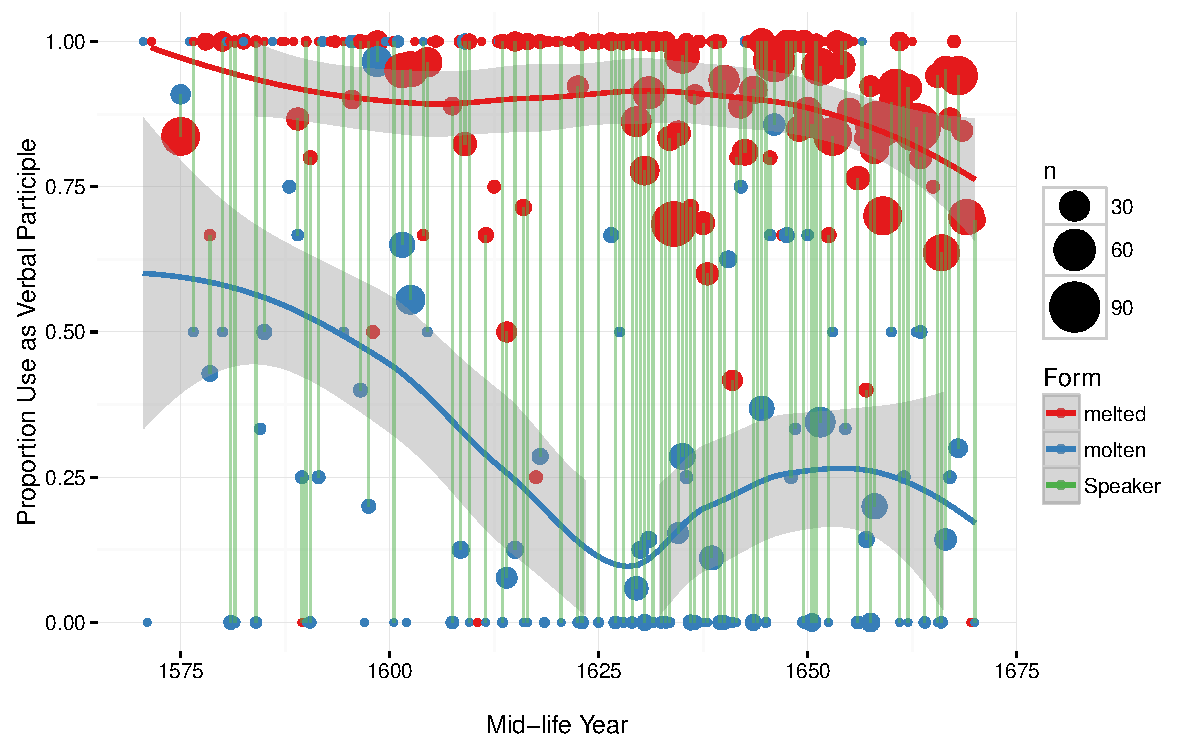
\includegraphics[scale=.6]{ContextByDateAuthor1570.pdf}
    \caption{Individual author \textsl{melted/molten} systems between 1570-1670.}
       \label{molten4}
    \end{center}
\end{figure}


\end{document}







 